\documentclass[12pt,fleqn]{article}\usepackage{../common}
\begin{document}
En Yakin k-Komsu (k-Nearest Neighbor)

Yapay Ogrenim alaninda ornek bazli ogrenen algoritmalardan bilinen kNN,
egitim verinin kendisini siniflama (classification) amacli olarak kullanir,
yeni bir model ortaya cikartmaz. Algoritma soyle isler: etiketleri bilinen
egitim verisi alinir ve bir kenarda tutulur. Yeni bir veri noktasi
gorulunce bu veriye geri donulur ve o noktaya ``en yakin'' k tane nokta
bulunur. Daha sonra bu noktalarin etiketlerine bakilir ve genellikle
cogunlugun etiketi ne ise, o etiket yeni noktanin etiketi olarak kabul
edilir.

``En yakin'' sozu bir kordinat sistemi cagristirir ve evet, kNN, aynen
k-Means ve diger pek cok sayisal bazli ogrenme yontemi gibi, eldeki cok
boyutlu veri noktalarinin elemanlarini bir kordinat sistemindeymis gibi
kabul eder. Kiyasla mesela APriori gibi bir algoritma metin bazli veriyle
oldugu gibi calisabilir. 

Bir veri obegi icinden en yakin noktalari bulmanin en basit yolu bu listeyi
bastan sonra taramak (kaba kuvvet yontemi -brute force-) ve her listedeki
nokta ile yeni nokta arasindaki mesafeyi teker teker hesaplayip en yakin k
taneyi icinden secmektir. Fakat bu islem de hizlandirilabilir. 

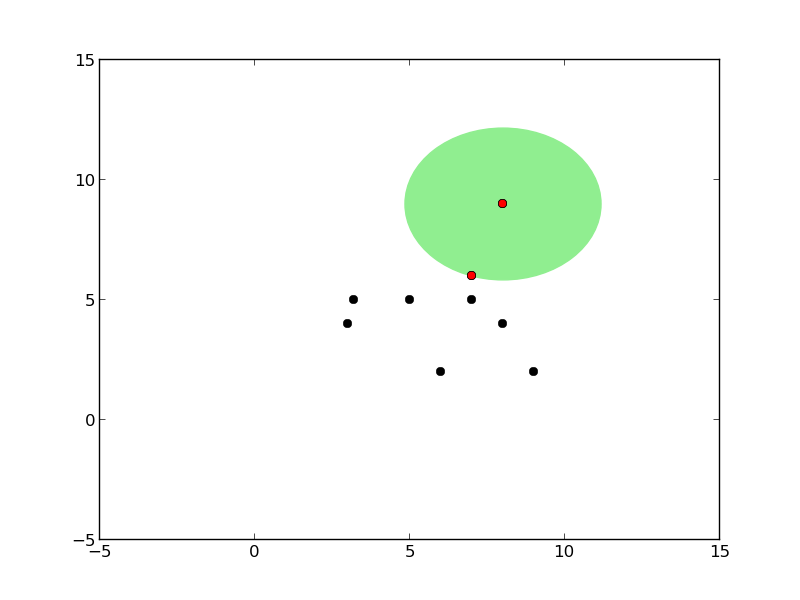
\includegraphics[height=7cm]{knn1.png}







\end{document}
